\documentclass[UTF8,fontset=fandol,a4paper,11pt]{ctexart}
\usepackage[left=2.35cm,right=2.35cm,top=2.35cm,bottom=2.35cm]{geometry}
\usepackage{amsmath,amssymb,booktabs,graphicx,float,tabularx,longtable,array,enumitem,hyperref,caption}
\hypersetup{hidelinks}
\setlength{\parindent}{2em}
\setlength{\parskip}{0.18em}
\setlength{\emergencystretch}{2em}
\newcommand{\pos}[1]{\left(#1\right)^+}
\newcommand{\keywords}[1]{\par\noindent\textbf{关键词：}#1}
\title{含光伏与储能微网的风险合同优化与反馈执行研究}
\author{}
\date{}

\begin{document}
\maketitle
\thispagestyle{empty}
\begin{abstract}
针对含光伏和储能的小区微网购电计划问题，本文建立“周期预测—残差风险修正—合同层线性规划—真实反馈执行—结算评价”的分层框架。每天划分为144个10分钟时槽；日前合同只使用历史数据、0时可得预测和历史误差统计，真实负荷与光伏仅在所属时槽到达后用于状态反馈。问题二的合同层将中心预测对应的基础合同与风险备用分开，以历史净负荷残差的0.8分位约束备用量，并以历史尾部短缺代理刻画5倍应急电价；执行层采用光伏、合同、储能、应急的确定性优先级，不再把MPC作为正式模型。MPC代码完整保留，仅在同一合同、预测与真实路径下用于执行策略对比。问题三、四继续考察日内调账和变动电价，并统一改用当前槽反馈执行。

典型日最优购电量为59482.70 kWh，费用35126.95元。2025年2月1日至12月31日334天中，问题二“风险合同LP+反馈执行”的总费用为1463.69万元，日均4.38万元，应急购电8.06万kWh。在逐日冻结同合同、同初始SOC和同信息的配对实验中，MPC对照费用为1642.04万元、应急45.25万kWh；反馈执行节省178.35万元。将预测误差标准差由\(0.5\sigma_0\)提高到\(2.0\sigma_0\)时，MPC与反馈执行的费用差由85.43万元扩大到317.44万元，表明后者在本数据和5倍应急电价下更稳定。问题三、四在严格相同0时信息的冻结合同基线上，日内调账分别节省37.56万元和39.99万元。未来扰动不变性实验中，两种执行器前48槽动作均保持不变；母线平衡最大残差为\(2.27\times10^{-13}\) kWh，未发生同时充放电。

\keywords{微网调度；储能；风险合同；线性规划；反馈执行；信息边界}
\end{abstract}

\newpage
\section{问题重述与总体思路}

微网每10分钟都要平衡负荷、光伏、储能与外部购电。合同买少时，真实缺口必须按基准电价的5倍应急购电；合同买多时，未使用部分又不能简单视为可全额退回。储能可以把能量从一个时段转移到另一个时段，但受容量、功率和效率约束。因此，本题不是单纯的峰谷套利，而是预测误差、合同条款、储能状态和信息发布时间共同作用的序贯决策。

四问按信息丰富程度逐层递进：问题一给定典型日的负荷、光伏和电价，建立确定性物理基线；问题二面对全年未知负荷和光伏，在每天0时一次性制定合同；问题三允许在6、12、18时读取新增光伏预报并调整尚未执行的合同；问题四进一步令电价随日期和时刻变化。本文在统一物理模型上依次增加预测、风险、调账和价格模块，总体路线为
\begin{equation}
\text{因果中心预测}\rightarrow\text{残差安全轨迹}\rightarrow\text{合同层LP}
\rightarrow\text{真实反馈执行}\rightarrow\text{现金结算与风险评价}.
\label{eq:route}
\end{equation}
式\eqref{eq:route}的各层职责不同：预测给出通常水平，风险层决定额外准备量，合同层给出可交易计划，反馈层只处理已经到达的真实偏差，结算层按题目条款计费。这一结构借鉴微网随机优化、模型预测控制与滚动时域规划的思想\cite{liang2014,hu2021,silvente2015}，但依据本题的信息结构选择较透明的风险合同LP与当前槽反馈作为正式机制。典型日结构见图\ref{fig:q1-raw}。

\begin{figure}[H]
  \centering
  
\includegraphics[width=0.94\textwidth]{figs/raw_q1_typical_profiles.png}
  \caption{典型日负荷、光伏和固定电价的日内结构}
  \label{fig:q1-raw}
\end{figure}

\section{数据处理、信息边界与基本假设}

\subsection{时间映射与统计范围}

每天含\(T=144\)个10分钟时槽。附件中的00:10表示00:00--00:10，24:00表示23:50--24:00，即表中标签视为区间终点。功率先换算为时槽电量：
\begin{equation}
E_{d,t}=P_{d,t}\Delta t,\qquad \Delta t=\frac16\ {\rm h}.
\label{eq:power-energy}
\end{equation}
全年计算从2025年1月1日开始，1月只用于预测冷启动和SOC连续推进；正式评价区间为2月1日至12月31日，共334天。

\subsection{数据清洗与一致性检查}

读入附件后，先将日期向下填充并把所有时刻统一为144个槽位；官方预报按“发布日期—发布时间—预报提前期”保存，不直接拼接到真实光伏列。随后依次检查日期连续性、每日槽数、负荷与光伏非负性、价格缺失和四个官方发布时间的完整性。功率列只在进入能量平衡前乘以\(1/6\)，避免同一变量在不同模块重复换算。

输出端逐槽重算母线平衡和SOC递推，逐日核对现金费用分项之和，并将汇总表与五份工作簿交叉比较。由此形成“原始数据—模型变量—逐槽结果—年度指标”的可追溯链，而不是只保留一个无法复核的总费用。

记日期\(d\)、调度时刻\(h\)可用的信息为\(\mathcal F_{d,h}\)。它包括此前日期的完整观测、当天\(h\)之前已经实现的负荷与光伏、截至\(h\)已经发布的官方预报，以及变价情形下已经实现的价格。\(h\)之后的真实负荷、光伏和价格均不属于\(\mathcal F_{d,h}\)。每次更新只能修改尚未执行的合同，已经执行的合同、能量流和SOC不允许回写。

\subsection{基本假设}

\begin{enumerate}[label=（\arabic*）]
  \item 微网不能向外部电网售电；光伏可供负荷、给储能充电或弃光。
  \item 储能容量为12000 kWh，SOC范围为1200--10800 kWh，充放电功率上限均为5000 kW，单向效率均为0.9。
  \item 问题一为循环典型日；问题二至四连续跨日推进SOC，不在午夜人为重置。
  \item 电价非负，不存在售电收入与储能吞吐补贴。主LP后用最小吞吐的次目标选择物理清晰的同费用解。
  \item 题面未给出储能老化、配网潮流、启停与需求响应数据，主目标不虚构这些货币成本。
\end{enumerate}

\section{统一物理模型与符号}

令\(\widetilde L_t,\widetilde V_t\)为一般规划子问题使用的负荷、光伏输入，\(g_t^{\rm P}\)为合同购电，\(v_t^{\rm P}\)为光伏利用量，\(x_t^{\rm P},y_t^{\rm P}\)为交流侧充、放电量，\(S_t^{\rm P}\)为规划SOC。问题一及问题三、四的合同更新子问题满足
\begin{align}
g_t^{\rm P}+v_t^{\rm P}+y_t^{\rm P}&=\widetilde L_t+x_t^{\rm P},\label{eq:plan-balance}\\
S_{t+1}^{\rm P}&=S_t^{\rm P}+\eta_cx_t^{\rm P}-y_t^{\rm P}/\eta_d,\label{eq:plan-soc}\\
0\le v_t^{\rm P}&\le\widetilde V_t,\quad g_t^{\rm P}\ge0,\nonumber\\
0\le x_t^{\rm P},y_t^{\rm P}&\le P_{\max}\Delta t,\quad S_{\min}\le S_t^{\rm P}\le S_{\max}.\label{eq:plan-bounds}
\end{align}

真实数据到达后，令\(g_t\)为该槽已生效合同，\(w_t\)为闲置合同，\(u_t\)为应急购电，带上标E的量为真实执行量，则
\begin{align}
g_t-w_t+v_t^{\rm E}+y_t^{\rm E}+u_t&=L_t+x_t^{\rm E},\label{eq:exec-balance}\\
S_{t+1}^{\rm E}&=S_t^{\rm E}+\eta_cx_t^{\rm E}-y_t^{\rm E}/\eta_d.\label{eq:exec-soc}
\end{align}
执行时先用光伏、再用合同满足负荷；若没有缺口，余光伏先充电、余合同再充电，剩余分别记为弃光和闲置；若仍有负荷缺口，则电池在SOC与功率约束内放电，最后才应急购电。应急电不允许给电池充电。应急量和闲置量是执行后的记账量，不是日前LP可以提前知道的变量。全年还满足\(S_{d+1,0}^{\rm E}=S_{d,144}^{\rm E}\)。

规划层与执行层分离可避免把事后量伪装为先验量。问题二日前LP使用历史短缺变量作为风险代理，但实际\(u_t,w_t\)仍只在回放执行后产生；规划代理不进入现金结算。因此“历史风险下的计划最优”和“真实路径上的费用较低”是两个命题，必须分别由LP与年度回测验证。

每个线性规划均用HiGHS求解。第一阶段最小化合同或调账成本，并给有限时域末端SOC保留价值；第二阶段在第一阶段目标值的数值容差内最小化\(\sum_t x_t+\sum_t y_t\)。这个字典序过程不改变经济最优值，只从多个等价解中选出吞吐较小、物理上更清晰的轨迹。全文主要符号及单位汇总见表\ref{tab:symbols}。

\begin{table}[H]
\centering
\caption{主要符号、单位和含义}
\label{tab:symbols}
\begin{tabularx}{\textwidth}{c c X}
\toprule
符号 & 单位 & 含义\\
\midrule
\(L_t,V_t\) & kWh & 真实负荷与可用光伏；带波浪号为规划安全轨迹\\
\(g_t,p_t,q_t\) & kWh & 生效合同、0时基准合同、最终调整合同\\
\(x_t,y_t,S_t\) & kWh & 充电量、放电量、储能电量\\
\(u_t,w_t\) & kWh & 应急购电与闲置合同\\
\(c_t\) & 元/kWh & 基准价格或真实结算价格\\
\(\alpha\) & -- & 净负荷安全分位水平，主设定为0.8\\
\(\mathcal F_{d,h}\) & -- & 日期\(d\)时刻\(h\)的可用信息集\\
\bottomrule
\end{tabularx}
\end{table}

\section{问题一：典型日确定性调度}

问题一的负荷、光伏和价格均已知，以购电费用最小为主目标：
\begin{equation}
\min C_1=\sum_{t=0}^{143}c_tg_t^{\rm P}.
\label{eq:q1objective}
\end{equation}
在式\eqref{eq:plan-balance}--\eqref{eq:plan-bounds}上施加循环约束。题面只要求0:00和24:00储电量相同；附件给出2025年1月1日0:00初始储电量为6000 kWh。因此先取\(S_0=6000\)，再由\(S_{144}=S_0\)推出\(S_{144}=6000\)。这不是额外假设“共同值必须是6000”，而是给定起点与循环条件的合并结果。

主目标达到最优后，在费用容差内进一步最小化\(\sum_t(x_t+y_t)\)。在非负电价、不可售电、无吞吐补贴的条件下，该次目标可从同费用解中排除无意义的同时充放电。若出现负电价、售电或补贴，则应改用含0--1互斥变量的混合整数模型。

总购电量为59482.698 kWh，费用35126.949元；充电20740.662 kWh，放电16799.936 kWh，弃光为0。SOC在1200--10800 kWh内运行，初末均为6000 kWh。循环条件还给出
\begin{equation}
\sum_t y_t=\eta_c\eta_d\sum_t x_t=0.81\sum_t x_t,
\label{eq:q1cycle}
\end{equation}
所以放电总量小于充电总量是效率损失的必然结果。母线平衡最大残差约为\(9.09\times10^{-13}\) kWh。图\ref{fig:q1-process}和图\ref{fig:q1-result}显示储能在低价或光伏富余时充电，在高价时段放电。

\begin{figure}[H]
  \centering
  
\includegraphics[width=0.91\textwidth]{figs/process_q1_price_dispatch.png}
  \caption{问题一电价与储能充放电时序关系}
  \label{fig:q1-process}
\end{figure}

\begin{figure}[H]
  \centering
  
\includegraphics[width=0.95\textwidth]{figs/result_q1_optimal_schedule.png}
  \caption{问题一最优购电、充放电与SOC轨迹}
  \label{fig:q1-result}
\end{figure}

\section{问题二：因果预测与日前合同}

\subsection{候选预测器与选型边界}

冻结的F1规则为：负荷取\(d-7\)日同槽值，光伏取前7个完成日同槽均值。另以旧90日加权模型F0和三周同星期中位数F2作误差对照。表\ref{tab:forecast}显示F1的净负荷MAE与RMSE最低，图\ref{fig:q2-process}展示其预测校验。当前证据只完成F0/F1/F2的预测误差对照和F1主线的年度闭环，故不声称三种预测器均已完成相同设置下的经济排名。

评价采用严格滚动起点：预测第\(d\)日时，残差库只包含第\(d-1\)日及更早观测。若\(e_i=\widehat P_i-P_i\)，则MAE为\(n^{-1}\sum_i|e_i|\)，RMSE为\(\,n^{-1}\sum_i e_i^2\,)^{1/2}\)。前者反映典型偏差，后者对少数大偏差更敏感；净负荷指标直接对应“负荷减光伏”的供电缺口，因此作为合同层的主要预测尺度。

\begin{table}[H]
\centering
\caption{三种因果预测器的误差对照（kW）}
\label{tab:forecast}
\begin{tabular}{lrrrrrr}
\toprule
模型 & 负荷MAE & 负荷RMSE & 光伏MAE & 光伏RMSE & 净负荷MAE & 净负荷RMSE\\
\midrule
F0 & 722.57 & 904.09 & 335.92 & 557.77 & 804.08 & 1074.83\\
F1 & \textbf{176.80} & \textbf{244.29} & 153.40 & 303.86 & \textbf{273.35} & \textbf{389.97}\\
F2 & 187.90 & 265.74 & 153.40 & 303.86 & 284.35 & 403.25\\
\bottomrule
\end{tabular}
\end{table}

\begin{figure}[H]
  \centering
  
\includegraphics[width=0.87\textwidth]{figs/process_q2_forecast_validation.png}
  \caption{问题二F1预测值与真实值的校验}
  \label{fig:q2-process}
\end{figure}

\subsection{残差风险修正与合同层LP}

设中心净负荷预测为\(\widehat N_t=\widehat L_t-\widehat V_t\)，历史净负荷残差定义为\(e^N_{j,t}=N_{j,t}-\widehat N_{j,t}\)。第\(d\)日0时只读取窗口\([\max(0,d-30),d)\)，不含第\(d\)日真实误差。若先忽略储能跨时耦合，单槽损失\(cp+5c\pos{N-p}\)给出\(\Pr(N>p)=1/5\)，故取\(\alpha=0.8\)作为风险备用分位。该推导只是价格驱动的边际风险标尺，不表示整日有80\%联合可靠度。

将合同拆为基础合同\(b_t\)与风险备用\(r_t\)，总合同为\(p_t=b_t+r_t\)。基础合同只平衡0时中心预测：
\begin{align}
b_t+v_t+y_t&=\widehat L_t\Delta t+x_t,\label{eq:risk-base}\\
r_t&\ge\max\{0,Q_{\alpha}(e^N_{\cdot,t})\Delta t\}.\label{eq:risk-floor}
\end{align}
对每个历史日\(j\)和时槽\(t\)，引入非负短缺代理\(z_{j,t}\)：
\begin{equation}
z_{j,t}\ge e^N_{j,t}\Delta t-r_t,\qquad z_{j,t}\ge0.
\label{eq:risk-shortfall}
\end{equation}
在SOC、功率及光伏约束下，合同风险目标为
\begin{equation}
\min\;\sum_t c_t(b_t+r_t)+5\sum_j\omega_j\sum_t c_tz_{j,t}
-\nu(S_T-S_{\min}).
\label{eq:risk-objective}
\end{equation}
末项是有限时域的终端SOC信用，只防止规划在日界处无价值地放空，不计入真实现金费用。代码分别记录基础合同费、备用合同费和历史尾部应急代理；实际结算只含已经购买的合同费用与真实应急费用。中心预测和历史残差均来自0时可见信息，真实未来负荷与光伏从未进入日前LP。

\subsection{当前槽反馈执行模型}

合同冻结后，第\(t\)槽只读取当前真实\(L_t,V_t\)和当前SOC。算法依次执行：光伏供负荷；合同补充负荷；无缺口时余光伏先充电、余合同再充电；有缺口时储能放电；最后不足部分应急购电。充电与放电分属互斥分支，且应急电不参与充电。执行结果代入式\eqref{eq:exec-balance}--\eqref{eq:exec-soc}更新SOC，并将日末状态连续传给下一日。

334日主模型总费用为14636893.76元，日均43823.04元；其中合同费用14142085.22元、应急费用494808.54元。应急购电80648.34 kWh，发生于456个时槽、136个连续事件；闲置合同2037924.81 kWh，弃光1557153.09 kWh。SOC始终位于1200--10800 kWh，期末为10800 kWh。全年结构及SOC连续性见图\ref{fig:q2-raw}、图\ref{fig:q2-soc}。

\begin{figure}[H]
  \centering
  
\includegraphics[width=0.96\textwidth]{figs/raw_q2_annual_netload.png}
  \caption{全年净负荷的季节—日内结构}
  \label{fig:q2-raw}
\end{figure}

\begin{figure}[H]
  \centering
  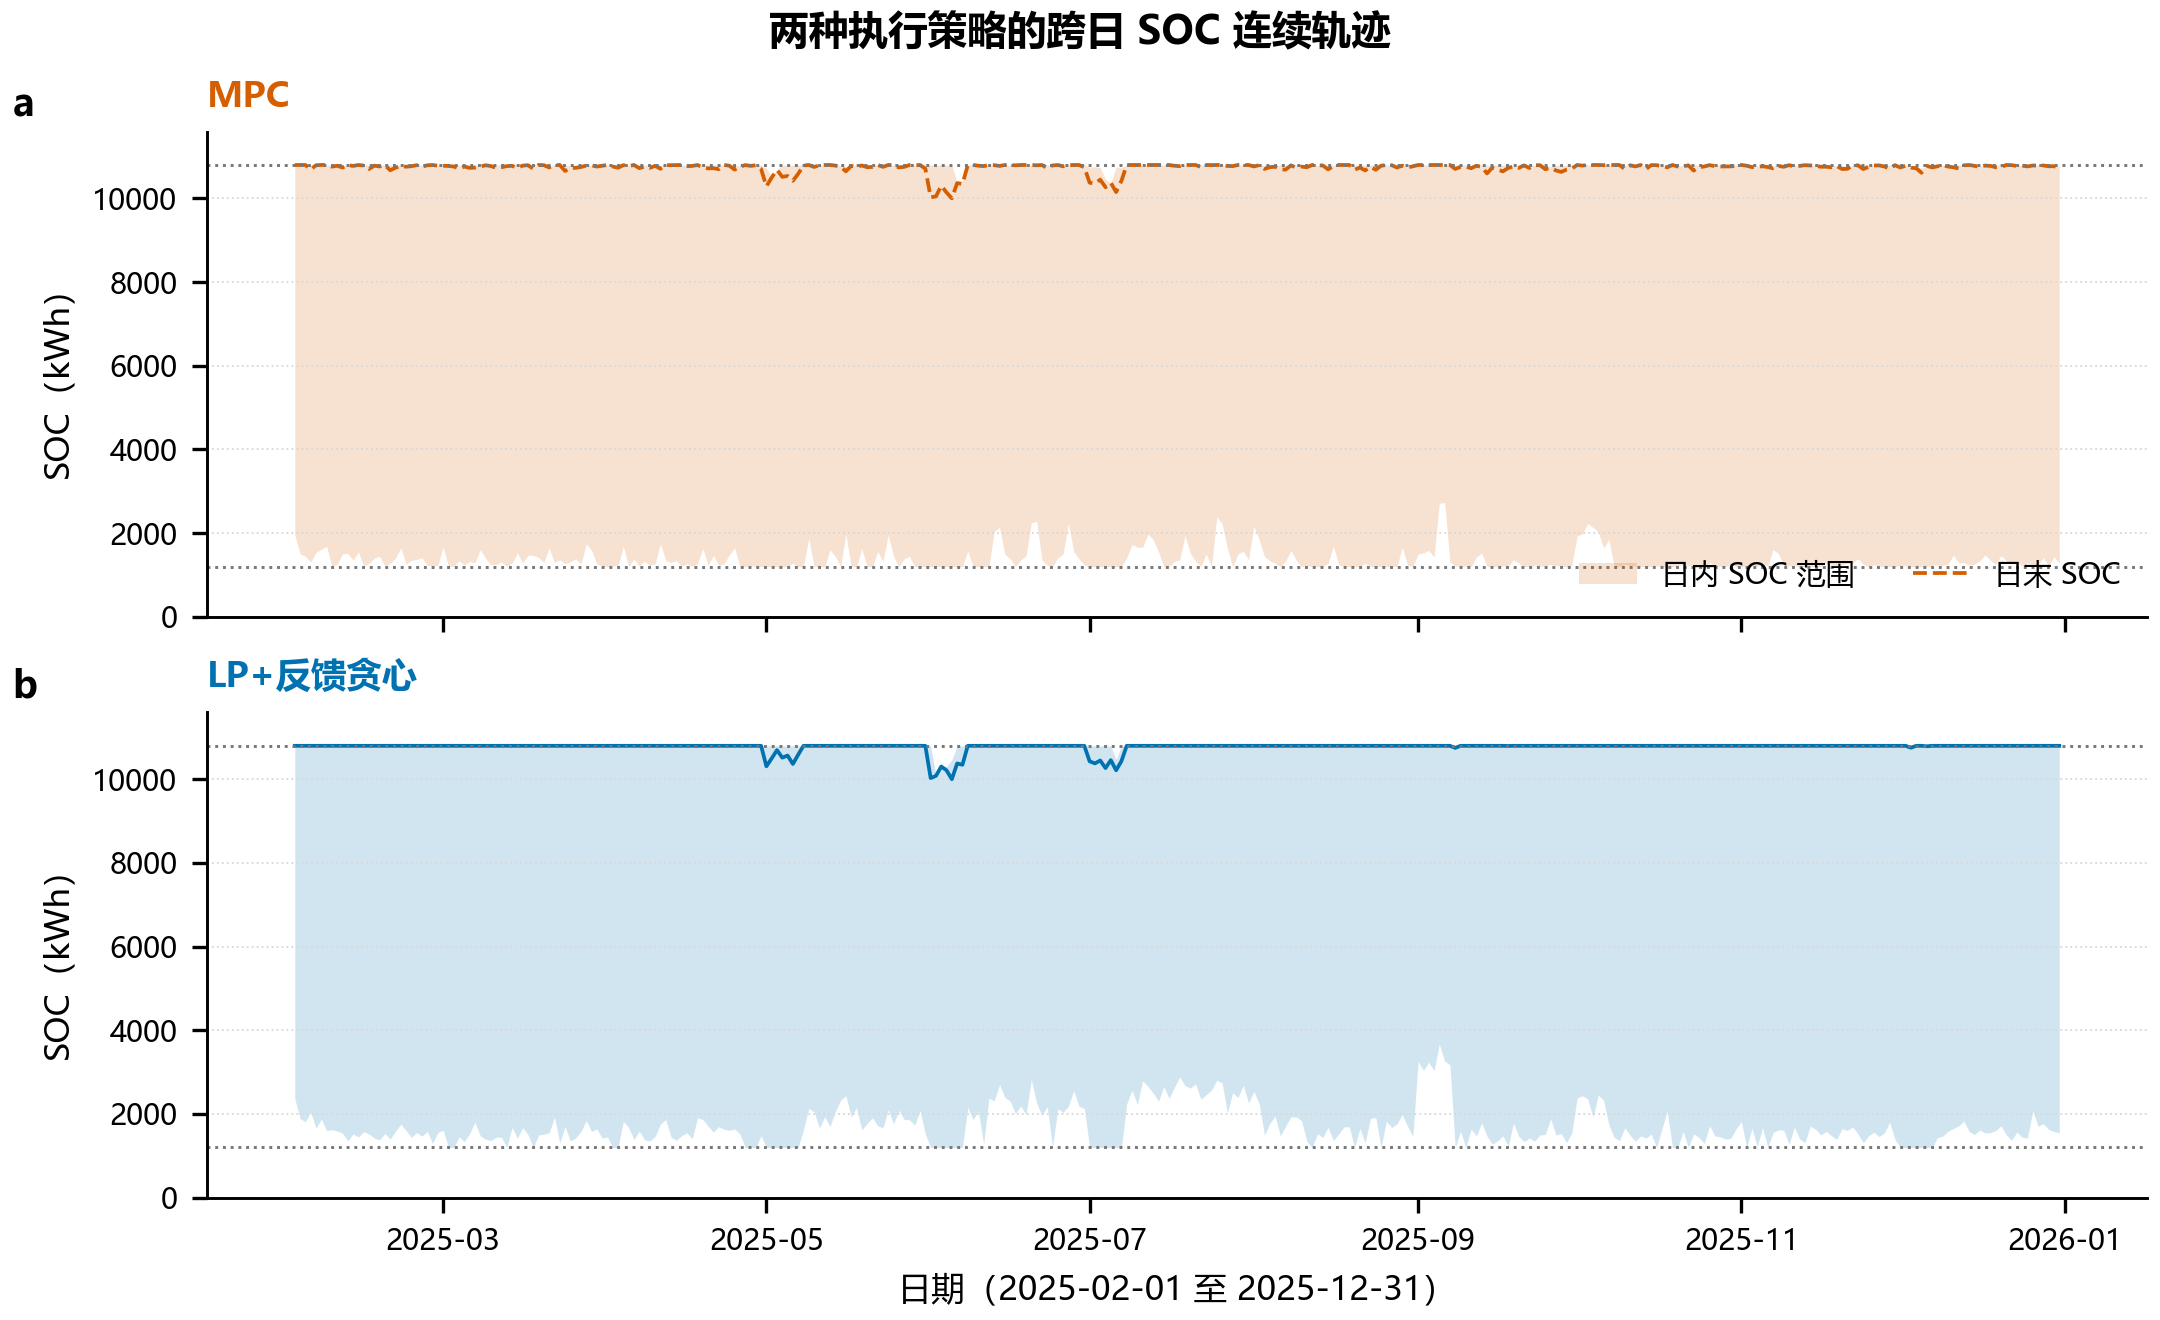
\includegraphics[width=0.95\textwidth]{figs/q2_soc_continuity.png}
  \caption{问题二两种执行策略的跨日SOC连续轨迹}
  \label{fig:q2-soc}
\end{figure}

\section{问题三：日内预报、合同调账与信息价值}

\subsection{滚动更新与结算}

0、6、12、18时发布的官方光伏预报先映射到10分钟网格，再用相同发布时间和提前期的历史偏差校准。每个事件以真实当前SOC为起点，重算尚未执行的合同；已执行前缀保持不变。日内能量流仍按问题二的当前槽反馈规则执行，而不是MPC。代表日合同变化见图\ref{fig:q3-process}。

\begin{figure}[H]
  \centering
  
\includegraphics[width=0.95\textwidth]{figs/process_q3_contract_updates.png}
  \caption{问题三代表日0、6、12、18时合同更新过程}
  \label{fig:q3-process}
\end{figure}

设0时基准合同为\(p_t\)，执行前最终合同为\(q_t\)，真实应急量为\(u_t\)。主结算为
\begin{equation}
C_t=c_t\left[\min(p_t,q_t)+1.5\pos{q_t-p_t}+0.5\pos{p_t-q_t}\right]+5c_tu_t.
\label{eq:settlement}
\end{equation}
若把原合同全额付费再叠加下调罚金，则\(q<p\)时费用为\(cp+0.5c(p-q)\)，下调越多反而越贵，并必然比不调整的\(cp\)高，不符合允许下调的经济含义。因此式\eqref{eq:settlement}作为主解释。替代式
\begin{equation}
C'_t=c_t\left[p_t+1.5\pos{q_t-p_t}+0.5\pos{p_t-q_t}\right]+5c_tu_t
\label{eq:altsettlement}
\end{equation}
仅用于同一物理轨迹重计费，不在替代规则下重新优化。

滚动过程按四步执行：0时生成全天基准合同\(p_t\)；更新事件到达时锁定已执行前缀；以当前真实SOC和最新可用预报重算剩余合同\(q_t\)及目标SOC；执行到下一事件并逐槽记账。对尚未执行的时槽，引入上、下调变量\(\delta_t^+,\delta_t^-\ge0\)，并令
\begin{equation}
b_t+r_t=p_t+\delta_t^+-\delta_t^-.
\label{eq:adjust-relation}
\end{equation}
更新LP沿用式\eqref{eq:risk-base}--\eqref{eq:risk-shortfall}的残差风险约束，将合同项改为
\begin{equation}
\min\;\sum_t c_t\bigl(p_t+1.5\delta_t^+-0.5\delta_t^-\bigr)
+5\sum_j\omega_j\sum_t c_tz_{j,t}-\nu(S_T-S_{\min}).
\label{eq:adjust-objective}
\end{equation}
由于同时增加同量的\(\delta_t^+\)和\(\delta_t^-\)会严格增加目标值，最优解不会同槽上、下调并存。末端SOC信用仍只服务于有限时域规划，不是现金收入。若把已经过去的槽位重新优化，算法会用新信息改写历史，费用虽可能更低，却不再是可实施策略。

\subsection{反馈执行下的调账结果}

反馈执行下，问题三日内调账主费用为14426279.48元，替代结算费用为15118551.31元；应急32292.76 kWh，闲置1579427.50 kWh，弃光1384142.51 kWh。其0时初始合同为22973737.44 kWh，逐次调整后生效合同为22141520.73 kWh。

为识别“允许6、12、18时调账”本身的净效应，另设\texttt{q3\_no\_adjust}：它与问题三共享0时官方预报、F1负荷预测、30个完成日残差、风险LP、初始SOC和反馈执行器，唯一差别是冻结0时合同。该严格基线费用为14801900.59元，应急80831.62 kWh，闲置2314004.19 kWh，弃光1540373.23 kWh。因此日内调账净节省375621.11元（2.54\%），并分别减少应急48538.86 kWh、闲置734576.69 kWh和弃光156230.72 kWh，见图\ref{fig:q3-result}。问题二与问题三还存在0时预报源差异，二者210614.28元的差额只能称为完整策略差异，不能解释为纯调账收益。

\begin{figure}[H]
  \centering
  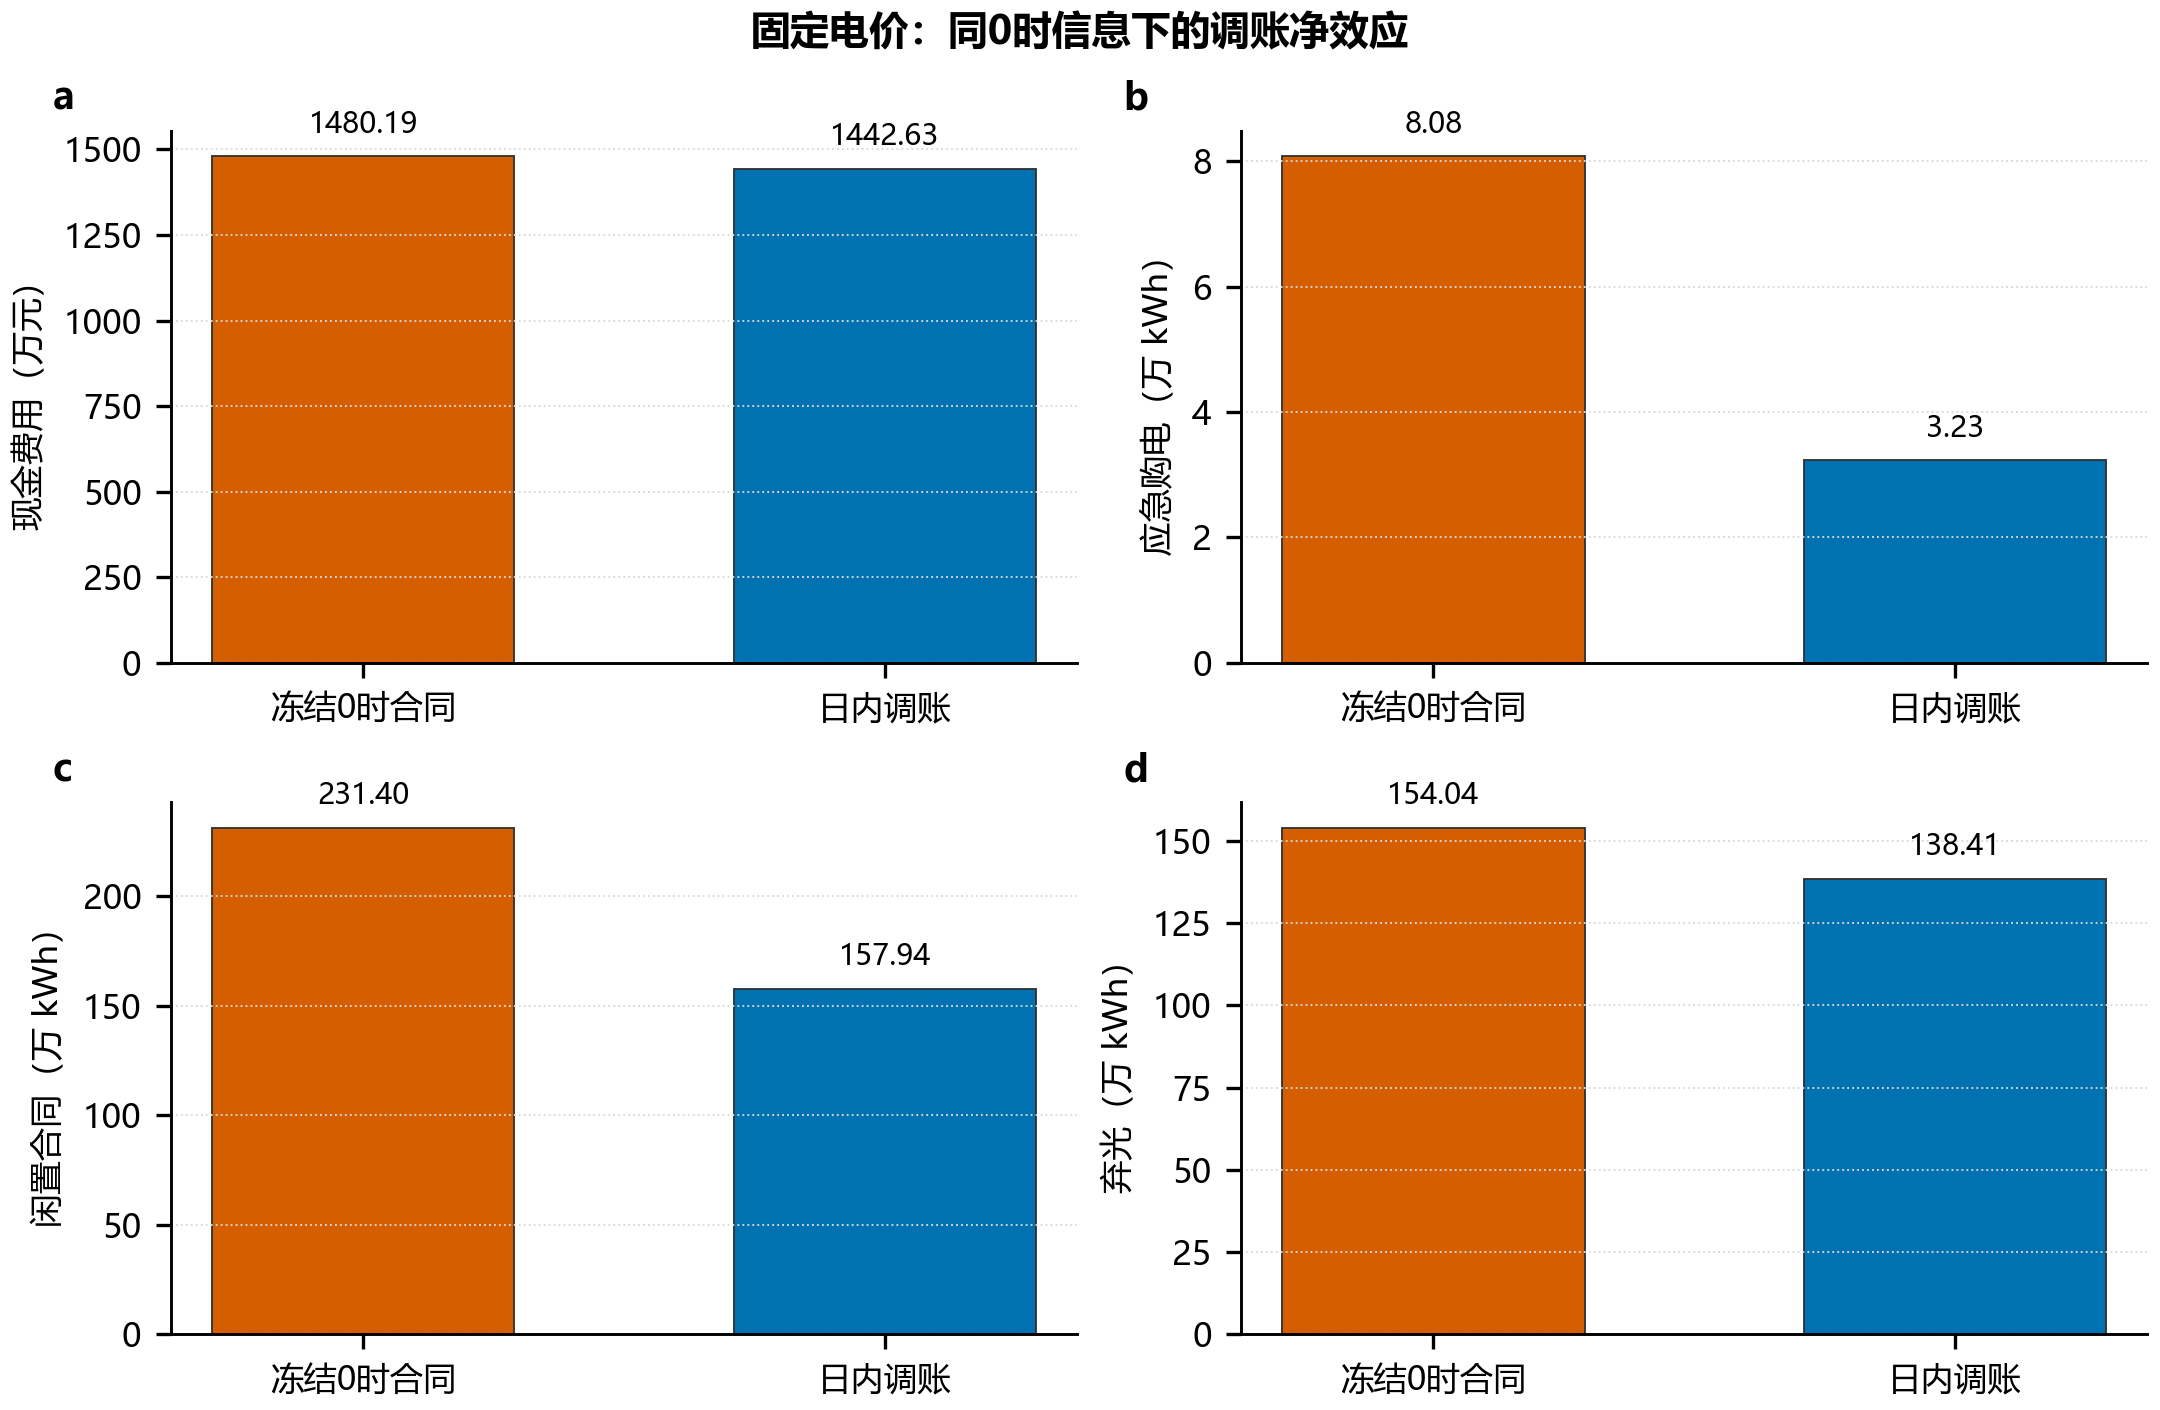
\includegraphics[width=0.93\textwidth]{figs/q3_greedy_adjustment_comparison.png}
  \caption{固定价下严格同0时信息的冻结合同与日内调账比较}
  \label{fig:q3-result}
\end{figure}

本次策略重构只将题目给定的0、6、12、18时发布信息用于合同更新；历史探索性批次不与新反馈基线混用。正文仅报告已按风险合同LP与反馈执行重新回测的题目分支，以及专门为因果识别新增的冻结合同基线。

\section{问题四：变动电价下的两种策略}

问题四若在0时直接读取全天真实价格，会产生完美未来信息。本文以过去30个完成日同槽价格中位数作为0时预测，并在日内用已实现价格偏差作指数衰减修正；未来真实价格只用于现金结算。价格波动和调度关系见图\ref{fig:q4-raw}、图\ref{fig:q4-process}。

\begin{figure}[H]
  \centering
  
\includegraphics[width=0.91\textwidth]{figs/raw_q4_price_variability.png}
  \caption{问题四真实电价的日内波动结构}
  \label{fig:q4-raw}
\end{figure}

\begin{figure}[H]
  \centering
  
\includegraphics[width=0.92\textwidth]{figs/process_q4_price_dispatch.png}
  \caption{价格预测、真实结算与储能调度的关系}
  \label{fig:q4-process}
\end{figure}

反馈执行下，问题四无调账分支费用15323615.30元，应急78919.00 kWh，闲置2006526.78 kWh，弃光1590815.54 kWh；有调账分支主费用15123873.94元，替代结算费用15837670.08元，应急31843.63 kWh，闲置1532390.95 kWh，弃光1413872.53 kWh。两题面分支的完整策略差额为199741.36元，但其0时光伏预报来源不同，不能直接当作纯调账贡献。

严格基线\texttt{q4\_3\_no\_adjust}与有调账分支共享0时预测、价格预测、残差、SOC和执行器，仅关闭日内调账；其费用为15523743.57元，应急80088.17 kWh，闲置2279304.66 kWh，弃光1577024.02 kWh。相对该基线，日内调账净节省399869.63元（2.58\%），应急、闲置和弃光分别减少48244.53、746913.72和163151.49 kWh。图\ref{fig:q4-result}给出严格配对结果，四个题面主分支见表\ref{tab:mainresults}。

\begin{figure}[H]
  \centering
  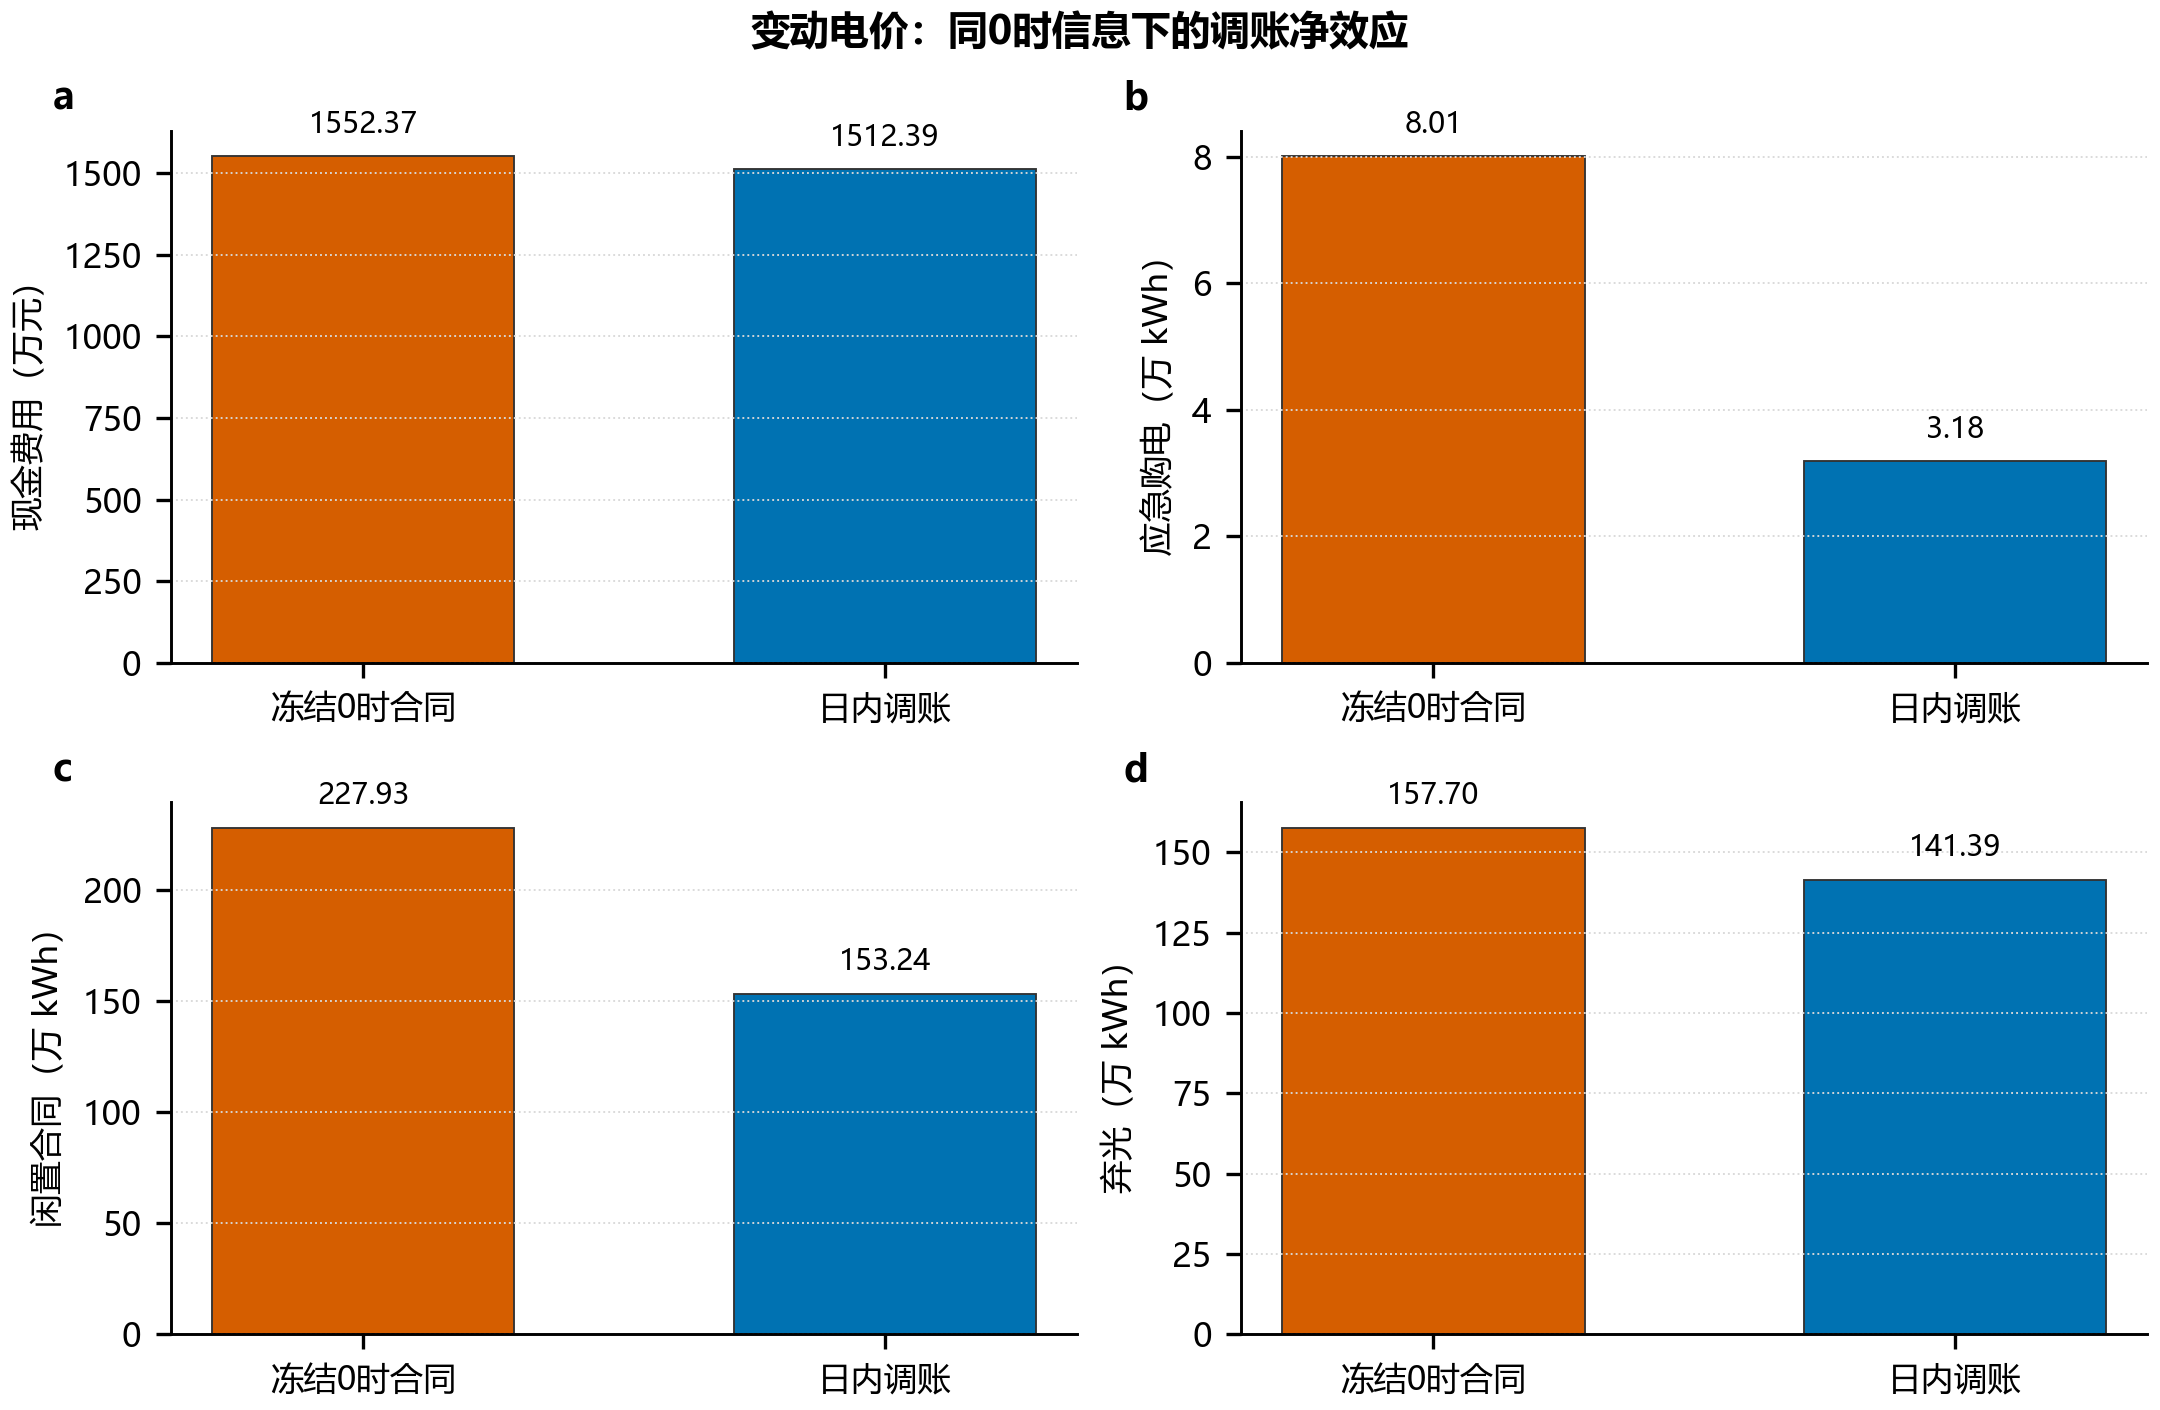
\includegraphics[width=0.92\textwidth]{figs/q4_greedy_adjustment_comparison.png}
  \caption{变动电价下严格同0时信息的冻结合同与日内调账比较}
  \label{fig:q4-result}
\end{figure}

\begin{table}[H]
\centering
\caption{334日四种年度主策略结果}
\label{tab:mainresults}
\resizebox{\textwidth}{!}{%
\begin{tabular}{lrrrr}
\toprule
策略 & 现金费用/元 & 应急/kWh & 闲置合同/kWh & 弃光/kWh\\
\midrule
问题二：固定价、0时合同 & 14636893.76 & 80648.34 & 2037924.81 & 1557153.09\\
问题三：固定价、日内调账 & 14426279.48 & 32292.76 & 1579427.50 & 1384142.51\\
问题四--2：变价、0时合同 & 15323615.30 & 78919.00 & 2006526.78 & 1590815.54\\
问题四--3：变价、日内调账 & 15123873.94 & 31843.63 & 1532390.95 & 1413872.53\\
\bottomrule
\end{tabular}}
\end{table}

\section{执行策略选择与验证}

\subsection{全年同信息集对比}

MPC保留为\texttt{baseline\_MPC()}，只作执行策略验证。配对实验逐日冻结反馈主线已生成的日前合同和日初SOC，并向两种执行器提供完全相同的预测路径、真实路径和结算价；MPC只使用已发布预测和当前SOC，反馈策略只在当前槽读取真实负荷与光伏。334日冻结同输入配对结果见表\ref{tab:controller}和图\ref{fig:q2-controller}。另行保留的各自连续跨日闭环仅作辅助诊断，不与本表的因果对照口径混用。

\begin{table}[H]
\centering
\caption{相同信息集下的334日执行策略比较}
\label{tab:controller}
\begin{tabular}{lrrrr}
\toprule
执行策略 & 总费用/元 & 应急/kWh & 闲置合同/kWh & 计算时间/s\\
\midrule
MPC对照 & 16420412.62 & 452547.46 & 2267443.46 & 375.186\\
LP+反馈执行 & 14636893.76 & 80648.34 & 2037924.81 & 0.156\\
\bottomrule
\end{tabular}
\end{table}

反馈执行减少费用1783518.86元（10.86\%），减少应急371899.12 kWh，执行计算约快2410倍。其原因并非使用更多真实信息，而是其动作直接响应当前供需和SOC，不依赖有限预测视野去跟踪未来目标SOC。依据当前数据、预测误差与5倍应急电价，反馈执行在费用、应急暴露和计算开销方面更适合作为正式运行策略；这一结论不外推为所有微网参数下的普适优越性。

\begin{figure}[H]
  \centering
  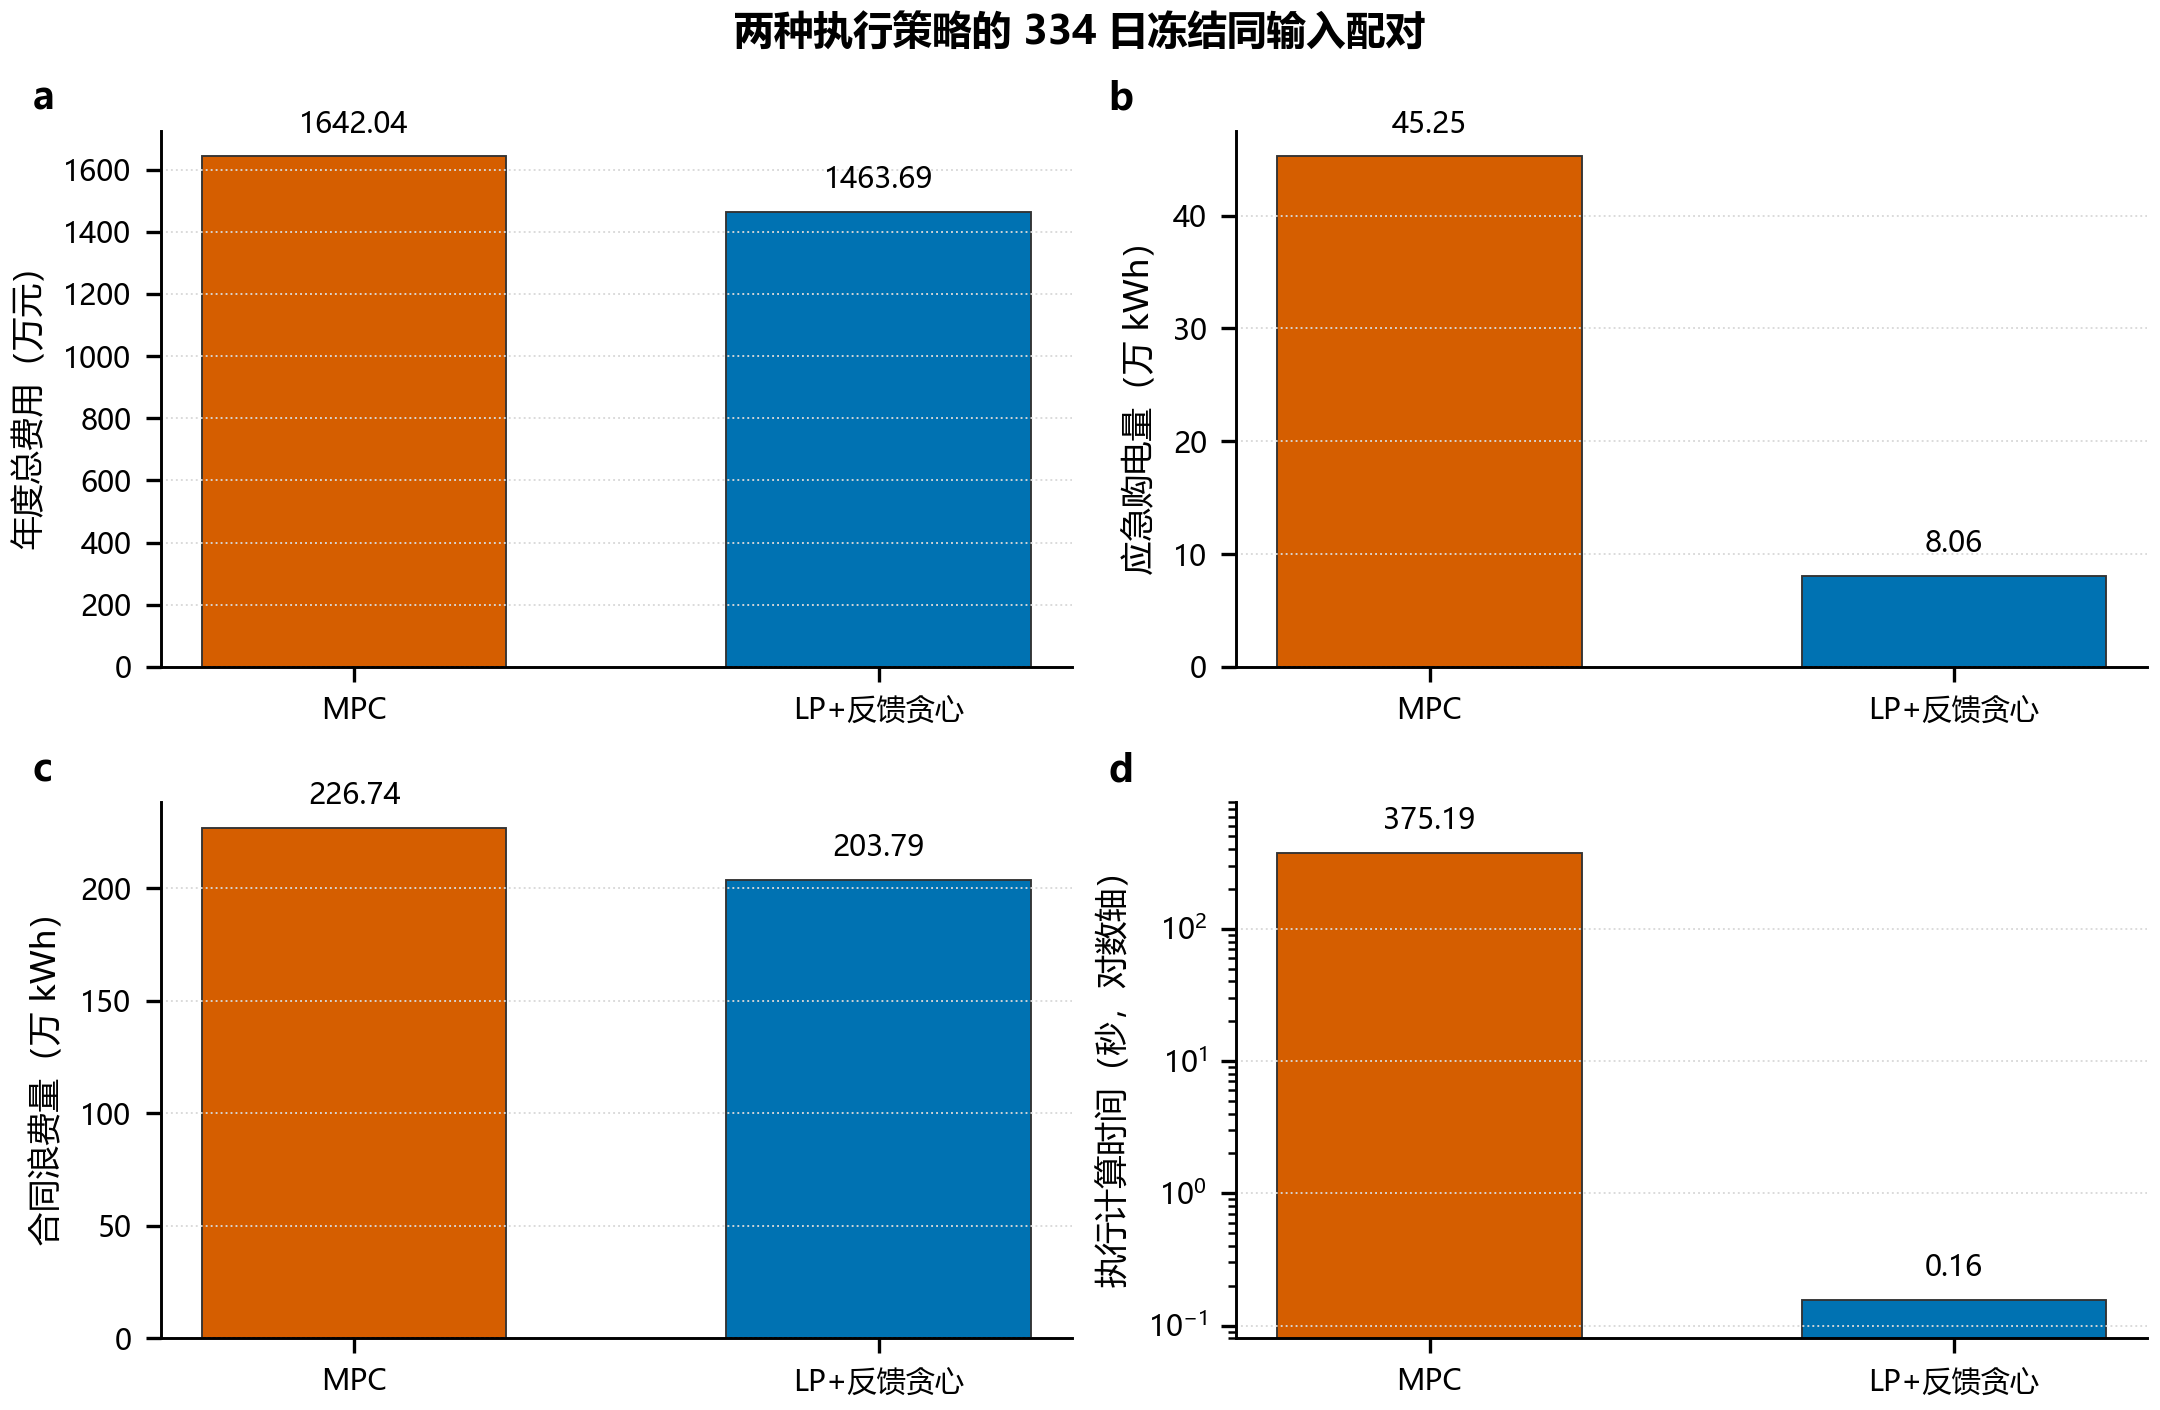
\includegraphics[width=0.95\textwidth]{figs/q2_execution_strategy_comparison.png}
  \caption{两种执行策略的334日冻结同输入配对}
  \label{fig:q2-controller}
\end{figure}

\subsection{预测误差敏感性}

固定日前合同和两种方法的信息集，将真实净负荷残差标准差调整为\(0.5,1.0,1.5,2.0\)倍基准。MPC与反馈执行的年度费用差依次为85.43、178.35、254.33和317.44万元；对应应急购电量分别由16.73/0.38万kWh增长到116.33/41.77万kWh（斜杠前后分别为MPC与反馈）。图\ref{fig:q2-error}显示误差增大时MPC的费用和应急暴露增长更快，反馈执行在本数据上的稳定性更好。

\begin{figure}[H]
  \centering
  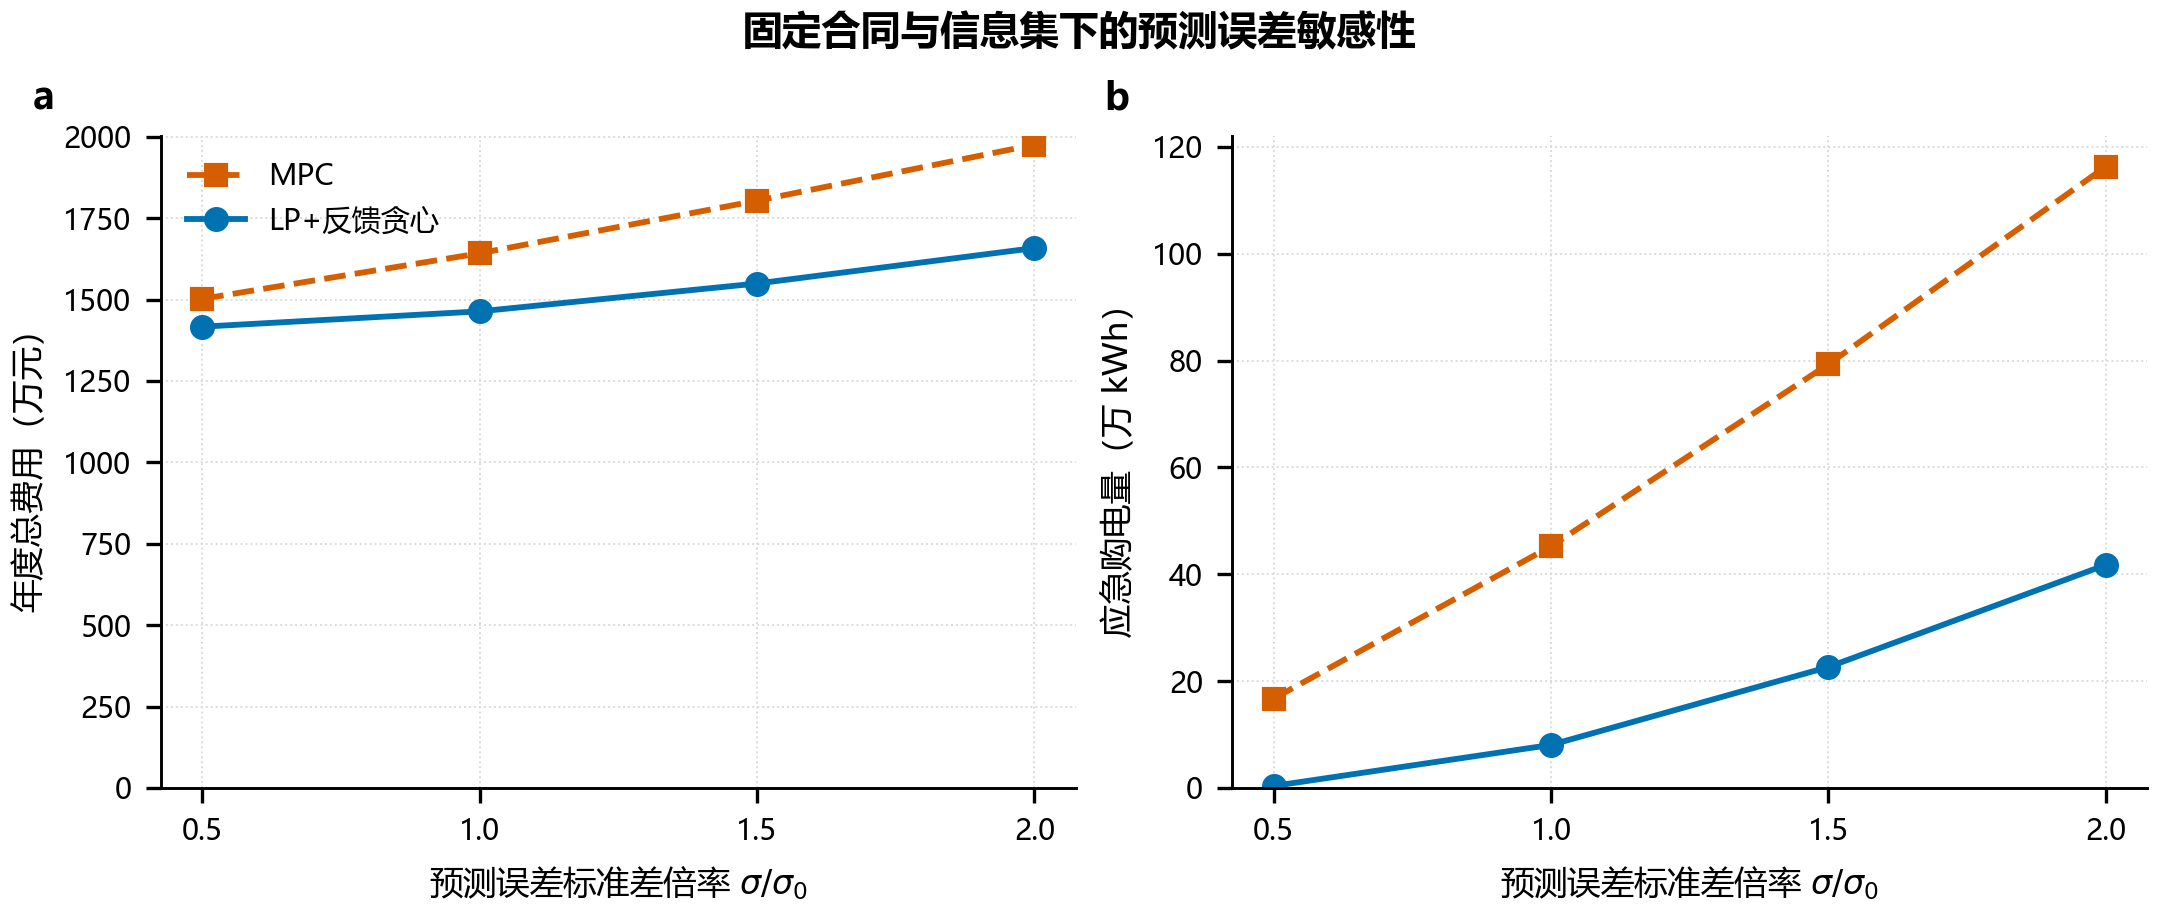
\includegraphics[width=0.95\textwidth]{figs/q2_error_sensitivity.png}
  \caption{固定合同与信息集下的预测误差敏感性}
  \label{fig:q2-error}
\end{figure}

\subsection{信息公平性与物理校验}

在2025年3月20日构造未来扰动实验，合同历史窗口固定为\([48,78)\)，将第48槽及之后的真实路径改变。日前合同最大差异为0，反馈与MPC前48槽动作及SOC最大差异均为0，证明“读取当前槽观测”不等于偷看未来。正式回测的SOC范围为1200--10800 kWh，同时充放电槽数为0，应急电充电槽数为0，最大母线平衡残差为\(2.27\times10^{-13}\) kWh。15项核心测试、结果评价测试和年度风险合同审计均通过。

\section{创新点、模型评价与适用边界}

本文的创新集中为三项：一是提出预测误差驱动的风险合同优化，将中心预测对应的基础合同、0.8分位风险备用和历史尾部短缺代理同时纳入LP；二是建立合同决策与真实执行解耦框架，使日前层遵守0时信息边界，执行层只用当前槽状态处理偏差；三是在相同合同、预测和真实路径下比较预测控制与反馈控制，并用全年回测、误差敏感性和未来扰动不变性形成可复核证据链。

模型透明、可追溯且计算稳定，但仍有边界：边际分位与历史短缺代理不能提供整日机会约束；F1依赖周周期，可能无法捕捉节假日和结构突变；反馈优先级没有显式电池老化成本，也不保证事后全局最优；储能退化、配电网潮流、需求响应和售电机制未进入模型。MPC对比只说明当前样本、参数和5倍应急电价下的适用性，不证明反馈控制普适优于预测控制。

\section{结论与实施建议}

问题一得到典型日费用35126.95元，并澄清6000 kWh来自给定初态与循环约束。问题二在F1预测、0.8风险分位和反馈执行下得到334日费用1463.69万元、应急8.06万kWh；相比冻结同合同、同日初SOC和同信息的MPC配对对照节省178.35万元，应急减少37.19万kWh。误差倍率升高时两者费用差持续扩大，支持将反馈执行作为本题正式策略。问题三固定价日内调账费用为1442.63万元；问题四变价日内调账费用为1512.39万元。与各自严格同0时信息的冻结合同基线相比，调账净节省37.56万元和39.99万元。

建议先以影子方式部署“0时风险合同+当前槽反馈”，逐日核对合同、SOC与结算，再在题目给定的官方发布时间开放合同调账。迁移到其他年份或微网时，应重新校准残差窗口、分位和终端SOC价值，并补充储能退化与网络约束；若误差结构或应急价格改变，应重新比较反馈与MPC的适用性。

\section*{AI工具使用声明}

本文参考稿在资料整理、代码审查、结果核对、LaTeX排版和语言润色阶段使用了人工智能辅助工具。模型、假设、结算解释、数据与结论须由参赛队伍结合原题和附件逐项理解、核验并承担最终学术责任。本文仅作为继续人工修改和复核的参考，不应在未经队伍审查的情况下直接提交。

\begingroup
\raggedright
\begin{thebibliography}{9}
\bibitem{liang2014} Liang H., Zhuang W. Stochastic Modeling and Optimization in a Microgrid: A Survey. \emph{Energies}, 2014, 7(4): 2027--2050. DOI: 10.3390/en7042027.
\bibitem{hu2021} Hu J., Shan Y., Guerrero J. M., et al. Model Predictive Control of Microgrids---An Overview. \emph{Renewable and Sustainable Energy Reviews}, 2021, 136: 110422. DOI: 10.1016/j.rser.2020.110422.
\bibitem{silvente2015} Silvente J., Kopanos G. M., Pistikopoulos E. N., Espu\~na A. A Rolling Horizon Stochastic Programming Framework for the Energy Supply and Demand Management in Microgrids. \emph{Computer Aided Chemical Engineering}, 2015, 37: 2057--2062. DOI: 10.1016/B978-0-444-63576-1.50081-9.
\end{thebibliography}
\endgroup

\newpage
\appendix
\section{冻结配置与复现说明}

主结果采用随机种子2026、F1预测、30日未聚类净负荷残差、\(\alpha=0.8\)和\texttt{greedy}反馈执行。问题二结果位于\path{results/q2_strategy}，问题三、四题面分支位于\path{results/q34_risk_contract_refactor}，严格冻结合同基线位于\path{results/q34_strict_baselines}。正式执行不使用MPC视野或SOC跟踪权重；36槽配置只属于\texttt{baseline\_MPC()}对比。复现入口为：
\begin{verbatim}
python -X utf8 run_q2_strategy_experiments.py
python -X utf8 run_all.py --project-root .
  --output-dir results/q34_risk_contract_refactor
  --variants q3 q4_2 q4_3 --controller greedy
python -X utf8 run_all.py --project-root .
  --output-dir results/q34_strict_baselines
  --variants q3_no_adjust q4_3_no_adjust --controller greedy
python -X utf8 audit_q34_risk_contract.py
\end{verbatim}

\section{结论使用边界速查}

本文支持“在本题样本、参数与同一信息集下”“反馈执行更适合作为正式策略”“调账分支已用新执行器重算”等条件化结论；不支持“完整随机MPC”“整日80\%可靠度”“反馈策略普适最优”“MPC失败”或“跨年份概率保证”等表述。

\end{document}
